\documentclass[11pt,a4paper]{article}
\usepackage[T1]{fontenc}
\usepackage[utf8]{inputenc}
\usepackage{lmodern,microtype}
\usepackage[margin=23mm,headheight=15pt,headsep=8mm,footskip=12mm]{geometry}
\usepackage{xcolor,graphicx,booktabs,tabularx,array,ragged2e}
\usepackage{listings,fancyhdr,titlesec,enumitem,amsmath}
\usepackage{tikz}
\usetikzlibrary{arrows.meta,positioning}
\usepackage[colorlinks=true,linkcolor=maroon,urlcolor=maroon,citecolor=maroon]{hyperref}
\definecolor{maroon}{HTML}{800000}
\definecolor{cream}{HTML}{F7F3ED}
\definecolor{muted}{HTML}{646464}
\hypersetup{pdftitle={LAlgo: Design and Validation of a Unified DFA Lexer},pdfauthor={PUP COSC 303 - Group 4}}
\setlength{\parindent}{0pt}
\setlength{\parskip}{6pt}
\emergencystretch=3em
\clubpenalty=10000
\widowpenalty=10000
\titleformat{\section}{\Large\bfseries\color{maroon}}{\thesection}{.7em}{}
\titleformat{\subsection}{\large\bfseries}{\thesubsection}{.7em}{}
\titlespacing*{\section}{0pt}{10pt}{8pt}
\titlespacing*{\subsection}{0pt}{10pt}{4pt}
\setlist{leftmargin=1.5em,itemsep=3pt,topsep=3pt}
\newcolumntype{Y}{>{\RaggedRight\arraybackslash}X}
\newcommand{\code}[1]{\texttt{#1}}
\newcommand{\callout}[1]{\par\smallskip\colorbox{cream}{\parbox{\dimexpr\linewidth-2\fboxsep\relax}{\small #1}}\par\smallskip}
\pagestyle{fancy}
\fancyhf{}
\fancyhead[L]{\small\color{maroon}\bfseries LAlgo / Unified DFA Lexer}
\fancyhead[R]{\small\color{muted}COSC 303 | Group 4}
\fancyfoot[L]{\small\color{muted}Implementation paper | 30 October 2026}
\fancyfoot[R]{\small\color{maroon}\thepage}
\renewcommand{\headrulewidth}{.3pt}
\lstset{basicstyle=\small\ttfamily,backgroundcolor=\color{cream},frame=single,
rulecolor=\color{cream},framesep=7pt,xleftmargin=8pt,xrightmargin=8pt,
breaklines=true,columns=fullflexible,keepspaces=true,showstringspaces=false,upquote=true}
\input{build/tests/summary.tex}
\begin{document}
\begin{titlepage}
\thispagestyle{empty}
\begin{center}

\includegraphics[width=25mm]{img/PUPLogo.png}\par
\vspace{4mm}
{\small REPUBLIC OF THE PHILIPPINES\par}
{\large\bfseries Polytechnic University of the Philippines\par}
{\normalsize College of Computer and Information Sciences\par}
{\normalsize Sta. Mesa, Manila\par}
\vspace{16mm}
{\fontsize{42}{46}\selectfont\bfseries\color{maroon}LAlgo\par}
\vspace{5mm}
{\LARGE\bfseries Design and Validation\par of a Unified DFA Lexer\par}
\vspace{5mm}
{\large Table-driven lexical analysis in C99\par}
\vspace{7mm}
{\color{maroon}\rule{65mm}{.7pt}\par}
\vspace{6mm}
{\small\bfseries GROUP 4 | BSCS 3-1\par}
\vspace{3mm}
Buenaventura, Harvey L.\par
De Mesa, Joshua C.\par
Dela Rosa, Mico Von Adriel A.\par
Magalona, Adriel M.\par
Morales, Timothy Gabriel\par
Nevado, Sean Andrew M.\par
Salvacion, Dean James G.\par
\vspace{7mm}
{\small Submitted to\par}
{\bfseries Prof. Ria A. Sagum\par}
\vspace{5mm}
Principles of Programming Languages (COSC 303)\par
\vfill
{\small Implementation snapshot | 30 October 2026\par}
\end{center}
\end{titlepage}
\setcounter{page}{1}

\section*{Abstract}
LAlgo is a proposed programming language for expressing algorithm-oriented source
programs. This paper documents its implemented lexical front end: a C99 scanner
that recognizes tokens using one deterministic finite automaton (DFA), one start
state, and one transition table. The selected implementation constructs 254
explicit states and 83 input classes. Reserved spellings are embedded in the
automaton through paired keyword-prefix paths, allowing uppercase recognition
and capitalization diagnostics without comparing completed lexemes against a
keyword list. A longest-match scanner adds source positions, newline metadata,
integer-range checks, and recovery for malformed input. Comments and invalid
lexemes remain visible in a token listing written to \code{Symbol Table.txt}.
A reproducible suite passes \ValidationPassed{} of \ValidationCases{} local
black-box cases, including the supplied positive and negative examples. These
results establish behavior for the tested lexical contracts; parsing, semantic
analysis, algorithm execution, and instructor acceptance are outside this study.

{\small\textbf{Keywords:} lexical analysis; deterministic finite automaton;
maximal munch; keyword trie; error recovery; C99.}

\section{Introduction and Implementation Scope}
A lexical analyzer converts source bytes into a stream of recognizable units.
For LAlgo, these units include names, constants, uppercase reserved words,
operators, punctuation, comments, and end-of-file. The practical requirement is
to make this recognition inspectable: each token can be traced to a path from
the same start state and to its original source location.

The earlier language proposal and subsequent lexical specification establish
the project context~\cite{spec,proposal}. This paper concentrates on the actual
selected program, \code{lexical\_analyzer/lalgo\_unified.c}~\cite{impl}.
The older \code{lalgo\_lexer.c} is retained as a historical implementation and
is not the implementation evaluated here.

\subsection{Objectives}
The implemented front end aims to recognize the specified token vocabulary,
distinguish keywords from identifiers using table transitions, preserve useful
source metadata, and report lexical errors while continuing where recovery is
defined. Its trace mode exposes state changes for explanation and inspection.

\callout{\textbf{Scope boundary.} Recognition of \code{WHILE}, \code{ARRAY}, or
\code{CARET} does not execute a loop, construct an array, or evaluate an exponent.
The sample programs demonstrate tokenization rather than executable language semantics.}

\clearpage
\section{Source and Token Contracts}
\subsection{Input and output}
The command line accepts a plain-text source file whose extension is
\code{.lal}; the extension check is case-insensitive. Embedded NUL bytes are
rejected before scanning. CRLF pairs are normalized to LF. An isolated carriage
return remains an invalid source byte. Space, tab, and LF are whitespace.
Locations begin at line 1, column 1; a tab advances one column rather than
expanding to a display tab stop.

Each token stores its type, original lexeme, starting line and column,
\code{precededByNewline}, and \code{suspectedKeyword}. The program prints a
token table and diagnostics, then writes \code{Symbol Table.txt} in the current
working directory. That file lists token occurrences, including repeated
identifiers, comments, and invalid lexemes; EOF is omitted from it.

\callout{The output filename uses ``Symbol Table,'' but the implemented data is
a lexical occurrence listing. It does not resolve declarations, scopes, types,
identifier uniqueness, or storage addresses.}

\subsection{Reserved spellings}
\begin{tabularx}{\linewidth}{@{}p{33mm}Y@{}}
\toprule Group & Uppercase spellings \\\midrule
Data types & \code{INTEGER DECIMAL CHARACTER BOOLEAN ARRAY STRING} \\
Control flow & \code{IF ELSE WHILE FOR} \\
Input/output & \code{INPUT OUTPUT} \\
Boolean constants & \code{TRUE FALSE} \\
Word operators & \code{DIV AND OR NOT} \\
Future-reserved & \code{ALGORITHM RETURN TRACE INVARIANT} \\
Noise words & \code{SET THE} \\\bottomrule
\end{tabularx}

The first five rows contain 18 current reserved spellings. Four future-reserved
words and two noise words bring the total to 24. The lexer emits noise-word
tokens; any later decision to omit them from an abstract syntax tree belongs
to a parser. Future-reserved tokens likewise carry no implemented runtime behavior.

\subsection{Identifiers and capitalization}
Identifiers follow \code{[A-Za-z][A-Za-z0-9\_]*}. An initial underscore is
invalid. Uppercase whole-word matches receive reserved token types.
\code{while} and \code{While} remain identifiers with
\code{suspectedKeyword=true}. \code{while1}, \code{WHILE\_}, and the incomplete
prefix \code{WHIL} are ordinary identifiers without that flag. The diagnostic
does not silently convert a name into a keyword.

\clearpage
\section{One Unified Deterministic Automaton}
\subsection{Representation}
Let $Q_e$ be the 254 explicit implementation states and let $\Sigma_c$ be
the 83 input classes, including virtual EOF. Recognition begins at $q_0$.
The program stores $\delta$ as \code{DELTA[state][class]} and records acceptance
in \code{ACC\_TOK}. Missing transitions use $-1$ and stop lookahead.
For a total mathematical DFA, add one implicit non-accepting sink $q_\bot$:
\[
M=(Q_e\cup\{q_\bot\},\Sigma_c,\delta,q_0,F),
\qquad \delta(q_\bot,c)=q_\bot.
\]
Thus 254 is the stored-state count, not the size of the totalized state set.
Acceptance actions distinguish token production, whitespace skipping, and
non-acceptance. The scanner emits EOF directly when no source remains.

\begin{center}
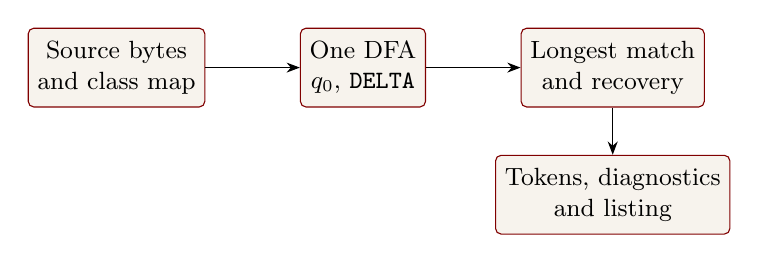
\begin{tikzpicture}[node distance=6mm and 12mm,>=Stealth,
box/.style={draw=maroon,rounded corners=2pt,fill=cream,align=center,font=\small,minimum height=10mm}]
\node[box] (bytes) {Source bytes\\and class map};
\node[box,right=of bytes] (dfa) {One DFA\\$q_0$, \code{DELTA}};
\node[box,right=of dfa] (scan) {Longest match\\and recovery};
\node[box,below=of scan] (out) {Tokens, diagnostics\\and listing};
\draw[->] (bytes)--(dfa);
\draw[->] (dfa)--(scan);
\draw[->] (scan)--(out);
\end{tikzpicture}
\end{center}
{\small\textbf{Figure 1.} Processing architecture. The boxes show program stages,
not independent token-recognition automata.}

\subsection{Classes and integrated keyword paths}
Each uppercase and lowercase letter has its own class, giving 52 letter
classes. The remaining 31 classes cover digits, relevant punctuation and
whitespace, other printable ASCII, illegal bytes, and EOF. A 256-entry map
classifies input bytes before transition lookup.

At startup, \code{build\_trie} constructs shared prefixes from the 24 reserved
spellings. Every non-root trie node becomes two DFA states: an exact-uppercase
state \code{E:prefix} and a folded-case state \code{F:prefix}. An exact terminal
accepts the corresponding reserved token. A folded terminal accepts an
identifier with the suspicion flag. Digits, underscores, or diverging letters
lead to a general identifier state, which continues the full name.

The keyword array is construction data. During scanning, keyword recognition
uses the same transition lookup as every other token family; it performs no
completed-lexeme string comparison. The generated full transition appendix in
the companion specification can be recreated using
\code{lexical\_analyzer/export\_unified\_dfa.py}~\cite{export}.

\clearpage
\section{Numbers, Literals, Operators, and Comments}
\subsection{Numbers and punctuation boundaries}
An integer is one or more digits; a decimal requires digits on both sides of
one dot. Leading zeros are accepted. Signs are separate tokens: \code{-2}
becomes \code{MINUS INTEGER}. Integer magnitudes above 2,147,483,647 generate
an \code{INVALID} token and a diagnostic. This range check runs after the DFA
recognizes the digit sequence.

\begin{tabularx}{\linewidth}{@{}p{30mm}Y@{}}
\toprule Input & Observed lexical result \\\midrule
\code{3.14} & One \code{DECIMAL} token. \\
\code{3.} & \code{INTEGER(3)}, then \code{DOT(.)}; lookahead backs up. \\
\code{.5} & \code{DOT(.)}, then \code{INTEGER(5)}. \\
\code{2low} & One malformed-number \code{INVALID} token. \\
\code{1.5abc} & One malformed-number \code{INVALID} token. \\
\code{1..2} & \code{INTEGER DOT DOT INTEGER}. \\\bottomrule
\end{tabularx}

The lexer preserves decimal text; it does not calculate or store a floating-point
numeric value. Numeric interpretation, expression precedence, and associativity
are later language-processing concerns.

\subsection{Quoted literals}
Strings use double quotes and may be empty. Character literals use single
quotes and require exactly one permitted body character. Both accept permitted
printable ASCII and tabs, while rejecting backslashes, LF, and illegal bytes.
There is no escape syntax. A quote matching the opening delimiter closes the
literal; the other quote character may appear in its body.

\subsection{Operators and delimiters}
Symbolic arithmetic tokens are \code{+ - * / \% \^{}}; \code{DIV} is the seventh
arithmetic operation's word token. Assignment is \code{=}; relational tokens
are \code{== != < <= > >=}. A lone \code{!} is invalid. Parentheses, square
brackets, braces, comma, semicolon, colon, and dot have individual accepting
states. A two-character operator supersedes its shorter accepted prefix under
the longest-match rule.

\subsection{Comment boundaries}
\code{//} consumes through the end of its line without consuming LF.
\code{/*} consumes through the first \code{*/}; block comments do not nest.
Comment bodies can traverse otherwise illegal bytes so the scanner can locate
the boundary, then report those bytes at their locations. Comments are retained
as auxiliary tokens. An unclosed block comment consumes the remaining input
as one invalid lexeme and produces an unterminated-comment diagnostic.

\clearpage
\section{Scanning, Metadata, and Recovery}
\subsection{Longest accepted prefix}
For each candidate, \code{dfa\_run} starts at $q_0$, advances through defined
transitions, and remembers the most recent accepting state and input length.
When a transition is missing, the scanner selects that remembered prefix.
The following pseudocode summarizes ordinary matching; committed errors are
handled before fallback.
\begin{lstlisting}
state = q0; offset = 0; last_accept = NONE
while DELTA[state][class_at(start + offset)] is defined:
    state = DELTA[state][class_at(start + offset)]
    offset = offset + 1
    if state has an accepting action:
        last_accept = (state, offset)
if stop_state is committed:
    recover malformed literal or block comment
else if last_accept exists:
    emit token, skip whitespace, or check numeric range
else:
    report and consume one illegal byte
restart at q0 for the next candidate
\end{lstlisting}

\subsection{Why committed states matter}
The slash in \code{/* open} is initially a valid division token. Once the
scanner enters the block-comment body, falling back to that slash would hide
the missing terminator. \code{COMMIT} marks open strings, character literals,
and block comments so an unfinished construct takes priority over an earlier
acceptance. Quoted-literal recovery consumes through a matching closing quote,
or stops before LF or EOF. Block-comment recovery consumes to EOF.

Malformed digit/name adjacency follows a separate accepting \code{BAD\_NUM}
path. Range failures convert a recognized integer candidate into
\code{INVALID}. Standalone illegal bytes consume one byte, ensuring progress.

\subsection{Newline metadata and diagnostics}
\code{advance} updates line and column positions for consumed input. Two
pending-newline flags distinguish normal tokens from auxiliary comment and
invalid tokens. An auxiliary row can display its own newline relationship
without erasing the flag needed by the next normal token. LF inside a consumed
block comment also affects the next token's metadata. These flags preserve
information; they do not implement statement boundaries.

Diagnostics include the offending construct's start position, or the specific
illegal-byte position within a comment. Exit status is 0 for a scan with no
lexical errors, 1 for a scan reporting lexical errors, and 2 for usage or file
handling failures. The command overwrites the listing on each completed scan.

\clearpage
\section{Worked Tokenization Example}
The following compact source illustrates uppercase recognition, a lowercase
keyword warning, decimal-dot backtracking, and newline propagation through a
comment. The displayed positions refer to normalized source text.
\begin{lstlisting}
INTEGER low = 3.
// boundary
while low <= 5
\end{lstlisting}

\begin{tabularx}{\linewidth}{@{}l l Y c c@{}}
\toprule Position & Token type & Lexeme & Newline & Suspected \\\midrule
1:1 & \code{KW\_INTEGER} & \code{INTEGER} & false & false \\
1:9 & \code{IDENT} & \code{low} & false & false \\
1:13 & \code{ASSIGN} & \code{=} & false & false \\
1:15 & \code{INTEGER} & \code{3} & false & false \\
1:16 & \code{DOT} & \code{.} & false & false \\
2:1 & \code{LINE\_COMMENT} & \code{// boundary} & true & false \\
3:1 & \code{IDENT} & \code{while} & true & true \\
3:7 & \code{IDENT} & \code{low} & false & false \\
3:11 & \code{LE} & \code{<=} & false & false \\
3:14 & \code{INTEGER} & \code{5} & false & false \\
4:1 & \code{EOF} & (empty) & true & false \\\bottomrule
\end{tabularx}
{\small\textbf{Table 1.} Expected stream for the example with a final LF.
EOF appears on screen and is excluded from the file listing.}

\subsection{Interpreting the paths}
For \code{INTEGER}, the automaton follows exact-uppercase prefix states and
ends at the reserved data-type token. For \code{while}, its lowercase first
letter selects a folded-case path; the completed spelling accepts \code{IDENT}
with the suspicion flag. If a digit were appended, the word would continue
into the general identifier state and lose that flag.

For \code{3.}, the digit state accepts an integer, then the dot reaches a
non-accepting decimal-prefix state. LF cannot complete the decimal, so the
scanner emits the earlier integer and restarts on the dot. For \code{<=},
the accepting less-than state extends to the accepting less-than-or-equal state.

\subsection{Connection to the supplied program}
\code{lexical\_analyzer/sample.lal} contains the illustrative binary-search
source. The current implementation produces 99 file-listing entries, including
one line comment, plus EOF on screen. Its zero lexical diagnostics demonstrate
successful recognition of the source. They do not establish that the program
parses, that its search terminates, or that LAlgo can execute it.

\clearpage
\section{Reproducible Local Validation}
\subsection{Method and results}
The test runner~\cite{tests} invokes the compiled executable in an isolated
temporary directory for each case. It checks the exit status, diagnostic count,
EOF presence, and listing contract. Cases add explicit token expectations or
metadata assertions where relevant. Expected token sequences are authored
independently of the DFA tables; the runner does not call internal recognition
functions. The source hash is recorded in \code{build/tests/results.json}.

\callout{\textbf{Measured result:} \ValidationPassed{} / \ValidationCases{}
local cases pass for the selected source snapshot. The build uses
\code{-std=c99 -Wall -Wextra -Wpedantic -Werror}. No performance benchmark or
exhaustive input-space proof is claimed.}

\begin{tabularx}{\linewidth}{@{}>{\RaggedRight\arraybackslash}p{35mm}Y@{}}
\toprule Contract area & Checks included in the suite \\\midrule
Reserved words & All 24 spellings, folded-case diagnostics, partial prefixes,
and suffixes that turn keywords into identifiers. \\
Names and numbers & Identifier alphabet, illegal initial underscore, leading
zeros, maximum integer, overflow, decimals, dot fallback, and number/name adjacency. \\
Punctuation & Arithmetic, assignment, relational operators, brackets,
delimiters, and lone-exclamation recovery. \\
Literals and comments & Empty strings, tabs, exact character length, forbidden
backslashes, unterminated constructs, non-nesting, and illegal comment bytes. \\
Positions and files & Newline across comments, CRLF normalization, tab columns,
isolated CR, empty input, file extension, NUL rejection, and trace dimensions. \\
Supplied examples & Positive binary-search sample, supplementary demo, and
negative example with seven diagnostics and seven invalid entries. \\\bottomrule
\end{tabularx}

\subsection{Evidence boundaries}
The tests verify selected observable behaviors, rather than every transition
or every possible malformed input. Exporting 254 states and 83 classes confirms
the implementation's current dimensions; it does not prove minimality of the
automaton. Token counts are specific to the supplied files and change when
their text changes.

The implementation retains the source, lexemes, and diagnostics in memory;
this is not a streaming interface. Very large files, allocation failure,
platform-specific integer and file-size limits, and timing behavior are not
covered by these checks. The report records local validation, not instructor
review, course grading, or external platform acceptance.

\clearpage
\section{Reproduction, Limitations, and Conclusion}
\subsection{Build and run}
From the repository root, run:
\begin{lstlisting}[language=bash]
make test
./build/lalgo lexical_analyzer/sample.lal
./build/lalgo lexical_analyzer/demo.lal t
./publish.sh --build-only
\end{lstlisting}
The first command compiles the selected C99 lexer and runs the contract suite.
The next two demonstrate ordinary output and optional DFA tracing. The last
command repeats validation, regenerates the full DFA appendix, and builds both
the language specification and this paper using Python 3 and a LaTeX installation
with \code{latexmk}. It does not publish to the papers website.

\subsection{Remaining work}
The lexer does not implement grammar recognition, type checking, scope
resolution, statement-boundary rules, precedence evaluation, or runtime
execution. Unicode identifiers, numeric exponent notation, escape sequences,
and nested comments are unsupported. Listing output is intended for inspection:
auxiliary lexemes are escaped and display-limited, and regular long lexemes can
widen the console layout. The listing is not a lossless serialization format.

Further work can define a parser contract around the existing token metadata,
specify semantics for current and future-reserved vocabulary, and broaden tests
with generated inputs. Those steps should preserve the distinction between
recognizing a source form and implementing its meaning.

\subsection{Conclusion}
LAlgo's current lexical front end combines token families and keyword prefixes
in one table-driven DFA. Longest-match selection handles shared prefixes,
while committed-state recovery prevents malformed quoted constructs and block
comments from disappearing into shorter tokens. Source positions, capitalization
flags, newline metadata, and auxiliary rows make its output inspectable. The
passing local suite provides a reproducible baseline for subsequent compiler work.

\begingroup\small
\renewcommand{\refname}{Project Sources}
\begin{thebibliography}{9}
\bibitem{impl} Group 4. \emph{Unified LAlgo lexical analyzer}. Repository source:
\code{lexical\_analyzer/lalgo\_unified.c}. Snapshot evaluated 30 October 2026.
\bibitem{spec} Group 4. \emph{LAlgo Language Design Specification}.
\code{lalgo\_language\_specification.tex}; companion PDF in this repository.
\bibitem{proposal} Group 4. \emph{Principles of Programming Language Proposal}.
Original proposal PDF retained in the repository.
\bibitem{export} Group 4. \emph{Unified DFA export utility}.
\code{lexical\_analyzer/export\_unified\_dfa.py}.
\bibitem{tests} Group 4 project repository. \emph{Lexer contract validation}.
\code{tests/test\_lexer.py}; reproducible report in \code{docs/VALIDATION.md}.
\end{thebibliography}
\endgroup
\end{document}
